\documentclass{beamer}
\usetheme{Madrid}
\usepackage{hyperref}

\title{Object extraction techniques and visual image search with Semantic web techniques}

\author[Aninda Maulik]{Aninda Maulik\\[10mm]{\small Supervisors: Prof. Pierre Maret \\ \hspace{18mm} Dennis Diefenbach}}
\institute[University Jean Monnet] % (optional)
{
  
  Cyber Physical and Social Systems\\
  University of Jean Monnet

}
\centering
\date{July 2020}
\begin{document}
\maketitle

\begin{frame}{Introduction:Just Google}
   \begin{itemize}
       \item images with bicycles
       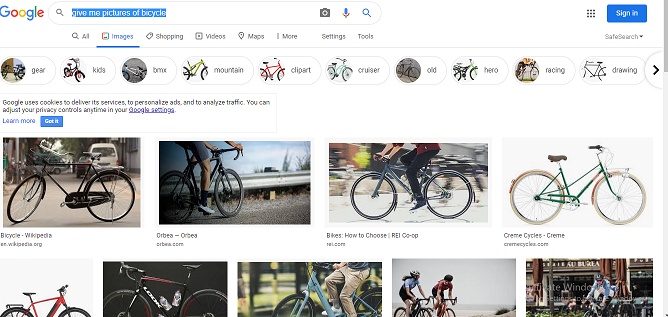
\includegraphics[]{googleBicycle.png}

\end{itemize}
\end{frame}

\begin{frame}{Google vs Qanswer}
   \begin{itemize}
       \item images with cars on the right
       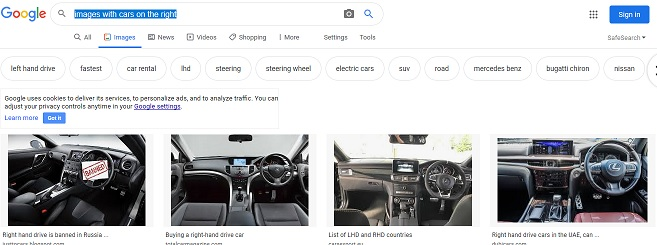
\includegraphics[]{google.jpg}

\end{itemize}
\end{frame}
    

\begin{frame}{Qanswer: images with car in the right}

       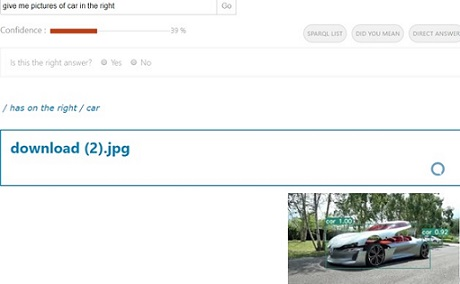
\includegraphics[]{carOnRight.jpg}


\end{frame}

\begin{frame}{Initialisation of work with a set of 22 images}

       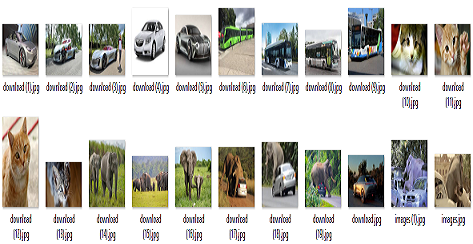
\includegraphics[]{22p80.png}


\end{frame}

\begin{frame}{special Wikimediacommons api give images }

\url{https://commons.wikimedia.org/w/api.php?action=query&list=search&srsearch=haswbstatement:P180=Q7378&srnamespace=6&format=json}
  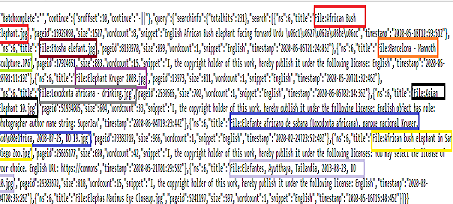
\includegraphics[]{wikimedia509075.png}     


\end{frame}

\begin{frame}{special Wikimediacommons api give human hand-annotated structured data}

\url{https://commons.wikimedia.org/wiki/File:African_elephants,_Lake_St_Lucia_06.jpg}
  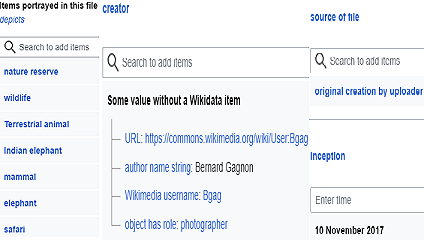
\includegraphics[]{structured7575.png}     


\end{frame}


\begin{frame}{special Wikimediacommons api give human hand-annotated structured data like copyright details}


  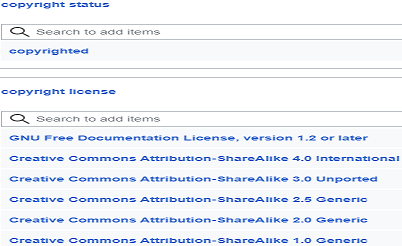
\includegraphics[]{copyright.png}     


\end{frame}

\begin{frame}{special Wikimediacommons api QID modified}


\url{https://commons.wikimedia.org/w/api.php?action=query&list=search&srsearch=haswbstatement:P180=Q5113&srnamespace=6&format=json}
  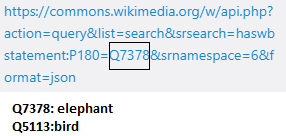
\includegraphics[]{wikimediacommons.png}     


    

\end{frame}
\begin{frame}{general API documentation link}
\url{https://www.mediawiki.org/wiki/API:Search}
\end{frame}
\begin{frame}{additional parameter introduced in the special Wikimediacommons api }

\url{https://commons.wikimedia.org/w/api.php?action=query&list=search&srsearch=haswbstatement:P180=Q7378&srnamespace=6&srlimit=500&format=json}
  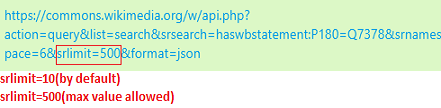
\includegraphics[]{srlimit.png}     


\end{frame}

\begin{frame}{additional parameter introduced in the special Wikimediacommons api and we get 231 images for Q7378 }

\url{https://commons.wikimedia.org/w/api.php?action=query&list=search&srsearch=haswbstatement:P180=Q7378&srnamespace=6&srlimit=500&format=json}
  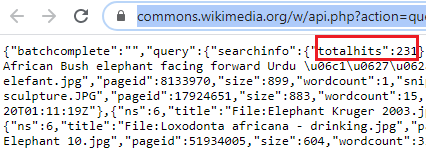
\includegraphics[]{totalhits.png}     


\end{frame}

\begin{frame}{special Wikimediacommons api gives more than 500 images for Q1420(car) }

\url{https://commons.wikimedia.org/w/api.php?action=query&list=search&srsearch=haswbstatement:P180=Q1420&srnamespace=6&srlimit=10&format=json&sroffset=10&continue=-||}
  
\includegraphics[]{217980.png}     


\end{frame}

\begin{frame}{additional parameter,sroffset, introduced in the special Wikimediacommons api and we iterate over}

\url{https://commons.wikimedia.org/w/api.php?action=query&list=search&srsearch=haswbstatement:P180=Q1420&srnamespace=6&srlimit=10&format=json&sroffset=10&continue=-||}
  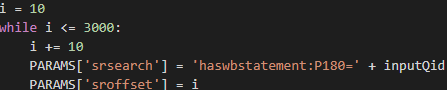
\includegraphics[]{iterate.png}     


\end{frame}
\begin{frame}{Qanswer: images with bicycle in the right}

       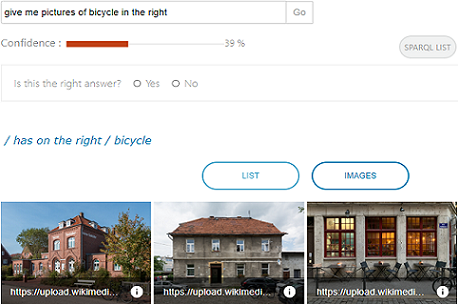
\includegraphics[]{right.PNG}


\end{frame}
\begin{frame}{set of bicycle images}

       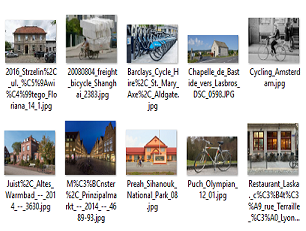
\includegraphics[]{bicycles.png}


\end{frame}

\begin{frame}{Qanswer: Image-Object Relation--contains}



  \begin{itemize}
      \item person and chair 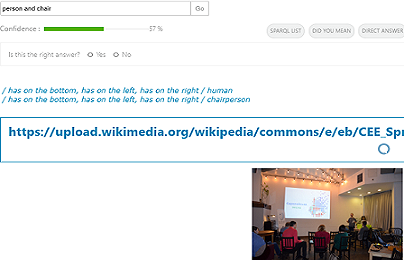
\includegraphics[]{personChair.png}

  \end{itemize}
 
\end{frame}

\begin{frame}{Content}
\begin{itemize}
\item Implementation of an Algorithm for object extraction. 
\item Design of a semantic web modelling for extracted data.
\item Implementation of a visual image search engine through Qanswer. 

\end{itemize}
\end{frame}

\begin{frame}{Implementation of an Algorithm for object extraction.}
\framesubtitle{YOLO-(You Only Look Once)}
\begin{itemize}
\item Implementation of an Algorithm for object extraction. 
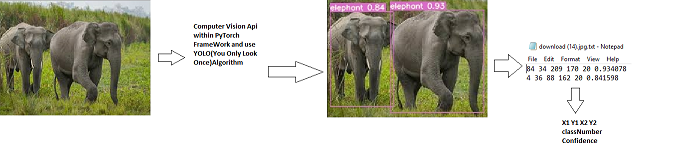
\includegraphics[]{pirated.png}
\end{itemize}
\end{frame}

\begin{frame}{Class Number, Class Name, QID}

\begin{itemize}
\url{https://github.com/pjreddie/darknet/blob/master/data/coco.names}
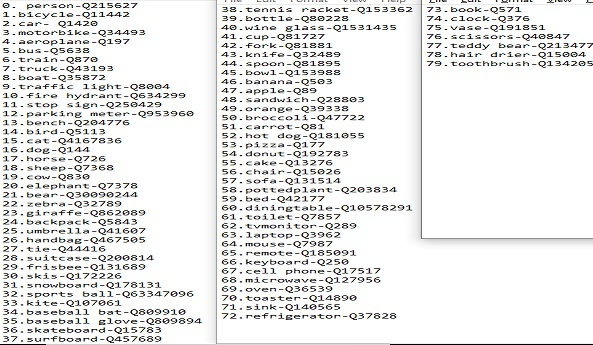
\includegraphics[]{classnameNumberQIDp.jpg}
\end{itemize}
\end{frame}


\begin{frame}{Bounding Box}


\includegraphics[]{b1.png}

\end{frame}


\begin{frame}{Co-ordinate representation of Bounding Box}


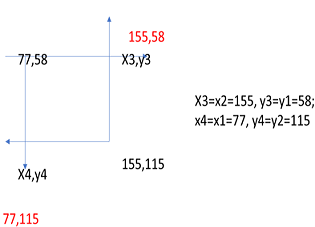
\includegraphics[]{b2.png}

\end{frame}



\begin{frame}{Image-Object Relations}


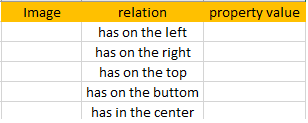
\includegraphics[]{tblrc.png}

\end{frame}


\begin{frame}{Algorithms for Image-Object Relations}


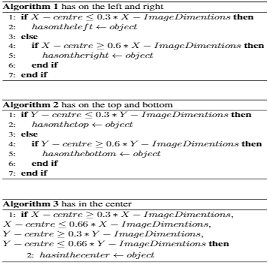
\includegraphics[]{algoIO.png}

\end{frame}

\begin{frame}{An attempt to show a graphical representation of tblrc}


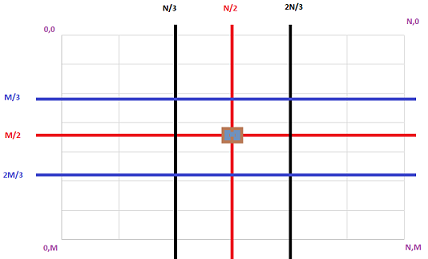
\includegraphics[]{tblrc chart.png}

\end{frame}

\begin{frame}{Using tblrc we create a csv file}


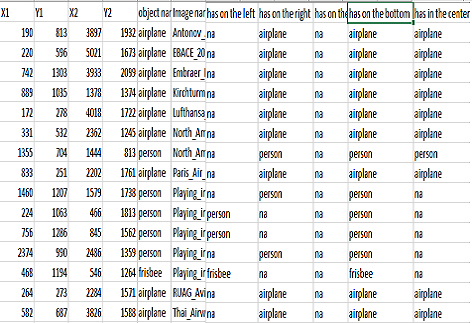
\includegraphics[]{ioCSV.png}

\end{frame}

\begin{frame}{Design of a semantic web modelling for extracted data.}
\framesubtitle{Image-Object Object-Object Relation}
\begin{itemize}
\item Design of a semantic web modelling based on the csv file.
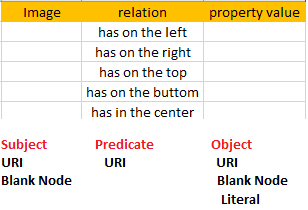
\includegraphics[]{tblrc2.png}
\end{itemize}
\end{frame}

\begin{frame}{Design of a semantic web modelling for extracted data.}
\framesubtitle{Image-Object Object-Object Relation}
\begin{itemize}
\item Design of a semantic web modelling for extracted data.
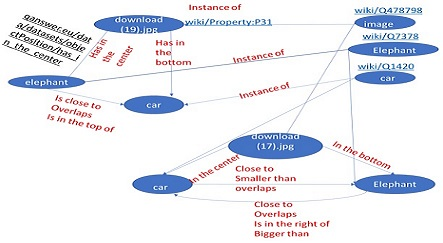
\includegraphics[]{semanticWeb.jpg}
\end{itemize}
\end{frame}

\begin{frame}{Thereafter we use the CSV file in a Java program and convert it into a RDF file}
\framesubtitle{Following this, we upload the file to QAnswer}
\begin{itemize}
\item QAnswer: airplane  in the center
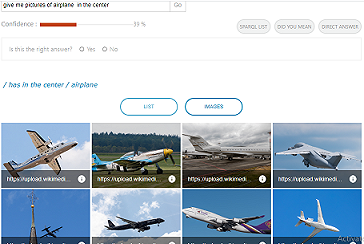
\includegraphics[]{airplaneQanswer.PNG}
\end{itemize}
\end{frame}

\begin{frame}{images in the left}
\framesubtitle{train in the left}

\begin{itemize}
\url{https://qanswer-frontend.univ-st-etienne.fr/user/query?kb=onto&user=anindamaulik}
\end{itemize}
\end{frame}

\begin{frame}{Automation pipeline}



  \begin{itemize}
      
      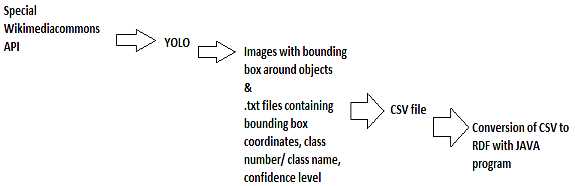
\includegraphics[]{automation.png}

  \end{itemize}
 
\end{frame}

\begin{frame}{Limitations and Future Work}
\framesubtitle{Query for images on the top}
\item Issue with confidence of detection by YOLO



  \begin{itemize}
      
      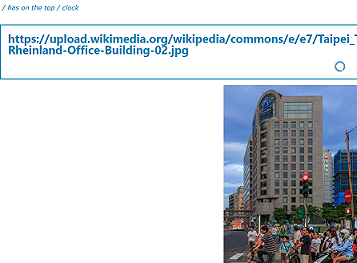
\includegraphics[]{top.PNG}

  \end{itemize}
 
\end{frame}
\begin{frame}{Contd..}
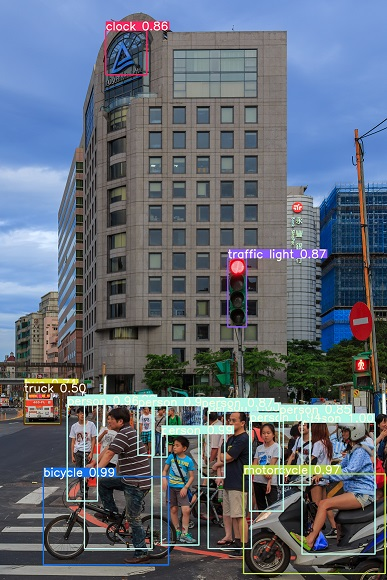
\includegraphics[]{bounding.jpg}

 
\end{frame}


\begin{frame}{Issue with the object name assigned by YOLO}
\framesubtitle{Traffic instead of Traffic Light}
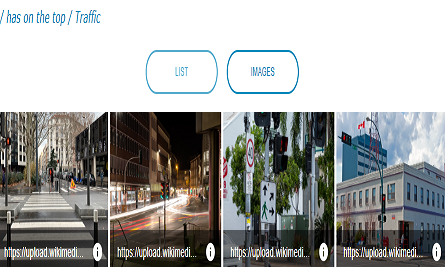
\includegraphics[]{topTraffic.PNG}

 
\end{frame}


\begin{frame}{Object-Object Relation}

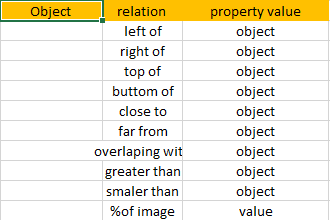
\includegraphics[]{OORelation.png}

 
\end{frame}


\begin{frame}{Reified Triple }

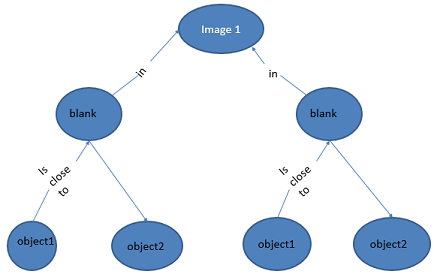
\includegraphics[]{reified.png}

 
\end{frame}

\begin{frame}{Reified Triple not being generated}

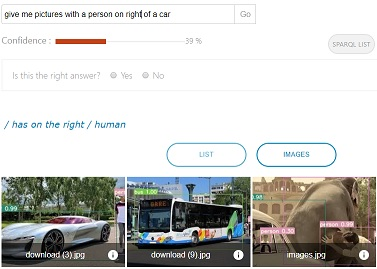
\includegraphics[]{objectObjectRelation(basics).jpg}

 
\end{frame}



\begin{frame}{OORelation algos ready to be used}



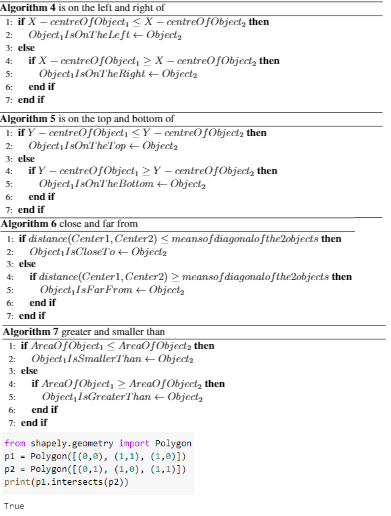
\includegraphics[]{ooalgo.png}

 
\end{frame}

\begin{frame}{Bounding Box}


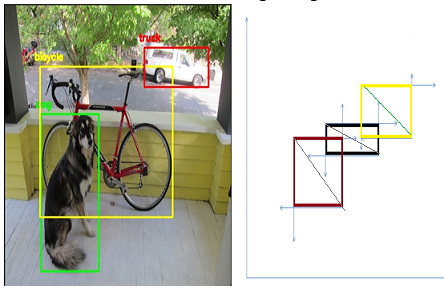
\includegraphics[]{diagonal.png}

\end{frame}

\begin{frame}{OORelation algos ready to be used, contd..}
\framesubtitle{Greater and Smaller Than}


      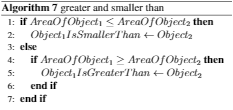
\includegraphics[]{ooalgo2.png}


\end{frame}

\begin{frame}{OORelation algos ready to be used, contd..}
\framesubtitle{Overlapping With}
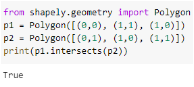
\includegraphics[]{overlapping.png}

 
\end{frame}

\begin{frame}{QAnswer issues}
\framesubtitle{Not getting the right query result}
\begin{itemize}
\item The wrong interpretation made due to non-availability of data
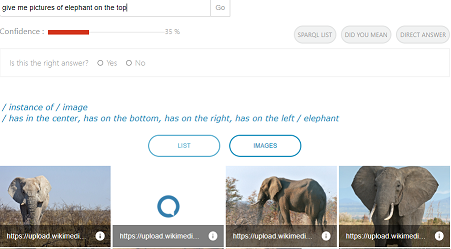
\includegraphics[]{QanswerElephantOnTheTopP.png}

\end{itemize} 
\end{frame}

\begin{frame}{In the csv file snapshot, we can see that there's data available, but not for elephant}

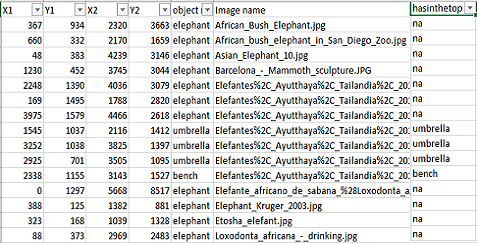
\includegraphics[]{elephantOnTheTopP.png}

 
\end{frame}

\begin{frame}{Failed to interpret the question correctly}
\framesubtitle{Carina}

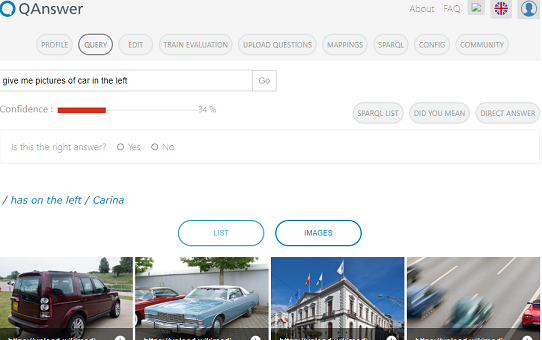
\includegraphics[]{carina60.png}

 
\end{frame}

\begin{frame}{END}



  \begin{itemize}
      \item Thank you for your attention, time and patience
      \item Please ask me any question that you have.
      \item Please provide your suggestion which can be used to make my work better
     

  \end{itemize}
 
\end{frame}

\end{document}
